\section{Type II Weyl semimetals}
\label{sec:typeii}

The conic section problem with the intersecting plane restricted to pass through the node of the cone is trivially seen to have two solutions: a point and two intersecting lines.
Despite this, the possibility of a Weyl cone tilted beyond the Fermi level was never considered before \citeauthor{soluyanovTypeIIWeylSemimetals2015} described this new class of Weyl semimetals in 2015.
This now seemingly obvious possibility made an already rich field even more exciting, opening up for a wider range of novel and interesting effects.
\todo{add some concrete examples or cites}

In the case of massless fermions, the particle physics equivalent of the Weyl semimetal, such a tilt is not possible, due to the requirement of Lorentz invariance \todo{add cite or explain}.
In condensed matter physics, however, this is not an issue, and it is indeed a real class of materials \todo{cite examples}.
We denote these types of materials Type-II Weyl semimetals, as opposed to Type-I.
The transition between Type-I and Type-II is abrubt -- the Fermi surface goes form a single point to two intersecting lines, in other words going from a zero dimensional to a one dimensional surface.
\todo{Make sure this is indeed a one dimensional surface. It is kind of 1DxZ(2)}
\todo{Make sure it is one dim also for the 3D case, quadric surface, not conic intersection}
Type-II also has electron and particle pockets at the Fermi level.
While the density of states for a Type-I semimetal goes to zero as one approaches the Fermi level, this causes Type-II to have a finite density of states at the Fermi level.
\todo{End with something like: all in all this gives type ii weyl semimetal manifestly different properties from tyep i, useful both in practical applications and as an interesting phenomena seen from a purely scientific perspective}

\subsection{Hamiltonian}
We will firstly consider a slightly more realistic toy model for a Weyl semimetal, with a parameter taking the system from a Type-I to a Type-II.
This is instructive both in order to more intuitively see the origin of the terms causing the tilting of the Dirac cone, and also to see how two Dirac cones in the same Brillouin zone tilt in relation to each other.
We will then continue by linearizing the model around the Weyl points, regaining the familiar form of a Dirac cone, with an additional anisotropy term causing the tilt.

Using the general time-reversal breaking model described by \citeauthor{mccormickMinimalModelsTopological2017} we have
\begin{equation}
  \begin{split}
    H(\vec{k}) &= \left[ ( \cos k_x + \cos k_z - 2 )m + 2 t (\cos k_x - \cos k_0) \right] \sigma_1\\
    &\pe - 2 t \sin k_y \sigma_2 - 2t \sin k_z \sigma_3
    + \gamma (\cos k_x - \cos k_0).
  \end{split}
\end{equation}
The model has Weyl nodes at \(\vec{K}' = (\pm k_{0}, 0,0)\), and the parameter $\gamma$ controls the tilting of the emerging cones.
A value of $\gamma=0$ gives no tilt, while for $\gamma > |2 t|$ the Type-II system emerges.
Figure \ref{fig:ridgeline} shows the cross section \(k_{y} = 0\) of the eigenvalues of this system, as \(\gamma\) is gradually increased from 0 to 0.15 \todo{verify numbers}.
The \(\gamma\)-term ``warps'' the bands, and in the limit of Type-II the hole band crosses the Fermi level into positive energy, while the particle band crosses the Fermi level into negative energies.
We call these hole and electron pockets, respectively.

Linearizing around the Weyl nodes reduces to the familiar expression of a Dirac cone
\begin{equation}
  \label{eq:32}
  H(\vec{K} ^{'\pm} + \vec{k}) \approx \mp 2 t k_{x} \sin k_{0} \sigma_{1} - 2 t (k_{y} \sigma_{2} + k_{z} \sigma_{3}) \mp \gamma k_{x} \sin k_{0} \sigma_{0}, \quad k_{x}, k_{y}, k_{z} \ll 1.
\end{equation}
When the separation between the two nodes is \(\pi\), i.e. \(k_{0} = \pi/ 2 \), the linearized Hamiltonian of around the cone, is
\begin{equation}
  \label{eq:33}
  H'(\vec{k}) = \mp 2 t k_{x} \sigma_{x} - 2t k_{y} \sigma_{y} - 2 t k_{z} \sigma_{z} \mp \gamma k_{x}.
  % h'(\vec{v}) = -2t \vec{k} \vec{\sigma} - \gamma k_{x}.
\end{equation}
However, as the two noes are brought closer together, the effective Fermi velocity in the \(x\)-direction is rescaled, and the system is anisotropic even for no tilt (\(\gamma=0\)).
The expression may be made even more clear by moving the sign \(\pm\)-sign into the tilt parameter \(\gamma\).
The Hamiltonian is invariant under a sign change of the first term, as the isotropic Dirac Hamiltonian is invariant under inversion.
In the tilt-term, we move the sign dependence into \(\gamma \), and the linearized model is
\begin{equation}
  \label{eq:34}
  H'(\vec{k}) = - 2t \vec{k} \vec{\sigma} - \gamma^{\pm} k_{x},
\end{equation}
where \(\gamma ^{\pm} = \pm \gamma \) with the upper sign corresponding to the node at \(k_{x} = + k_{0}\) and the lower sign corresponds to the node at \(k_{x} = - k_{0}\).
As expected, we get two Dirac cones, tilting in opposite direction, but with the same amount.
\todo{How does this affect the Berry curvature and chern number?}
\todo{Maybe prettier/more correct to invert ky and kz, as that would also give the opposite chirality of the dirac points}

The linearized model are accurate in describing low energy interactions around the Fermi level.
For higher energies their validity falls apart, and more complex models are warranted.
In our calculations the linear models is sufficient, and much easier to work with, and we will thus mainly consider the linear model from here on.

For tilted Dirac cones we will consider the Hamiltonian
\begin{equation}
  \label{eq:124}
  H =  s v_F \vec{k} \vec{\sigma} + v_F \vec{t}^s \vec{k},
\end{equation}
where \( s \) denotes the chirality of the Dirac cone, \( v_F \) is the Fermi velocity, and \( \vec{t} \) is the \emph{tilt vector}.
\todo{note about anisotropic Fermi velocity}
The tilt vector will in general depend on the chirality of the Dirac cone.
As the Dirac cones always appear in pairs, \( \vec{t}^s = s \vec{t} \) will give a system with inversion symmetry.
In the case of broken inversion symmetry, we will consider the case of a tilt equal in direction and magnitude between the two cones, \( \vec{t}^s = \vec{t} \).
In short, we define
\[
  \vec{t}^s =
  \begin{cases}
    \vec{t} & \text{broken inversion symmetry},\\
    s \vec{t} & \text{inversion symmetry}.
  \end{cases}
\]

With no magnetic field, the eigenvalues of the system are
\begin{equation}
  \label{eq:44}
  E(\vec{k}) = \vec{\omega_{0}} \vec{k} \pm \sqrt{(v_{i} k_{i})^{2}} = \sqrt{(t_{i} v_{i} k_{i})^{2}} \pm \sqrt{(v_{i} k_{i})^{2}},
\end{equation}
where in the literature the first term is sometimes referred to as the \emph{kinetic} term while the latter is the \emph{potential} term.
The definition for the system to be Type-II is that there exists a direction in momentum space for which the kinetic term dominates over the potential term \cite{soluyanovTypeIIWeylSemimetals2015}.
The \(\vec{t}\)-vector is thus a convenient tool for categorization -- if \(t > 1\) we have a Type-II, else we have a Type-I.
\begin{proof}
  We may always rotate our coordinate system such that, without loss of generality, \(\vec{t} = t \hat{x}\).
  In that case, the first term obviously dominates in the \(x\)-direction, when $t>1$.
\end{proof}

\begin{itemize}
  \item gives rise to cones tilting opposite direction
  \item Linearized model valid for low energy interaction. For higher energy, the perfect cone model is not valid, as the cones does in fact touch.
  \item In this model, the hole pocket is ``shared'' between the two cones. There are also models with individual pockets (see \cite{mccormickMinimalModelsTopological2017})
\end{itemize}

\begin{figure}[ht]
  \centering
  
\includegraphics[width=0.4\textwidth]{figures/conicSection}
  \caption{\label{fig:conic-section-sketch} }
\end{figure}


\begin{figure}[ht]
  \centering
  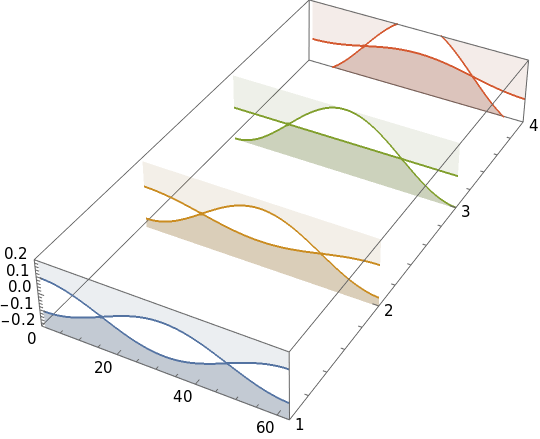
\includegraphics[width=0.7\textwidth]{figures/typeIIridgeline}
  \caption{\label{fig:ridgeline} \todo{Write this} The values of the parameters were chosen to be \(m=0.15, t=-0.05, \) and \(2 k_{0}=\pi\).}
\end{figure}

\begin{figure}[ht]
  \centering
  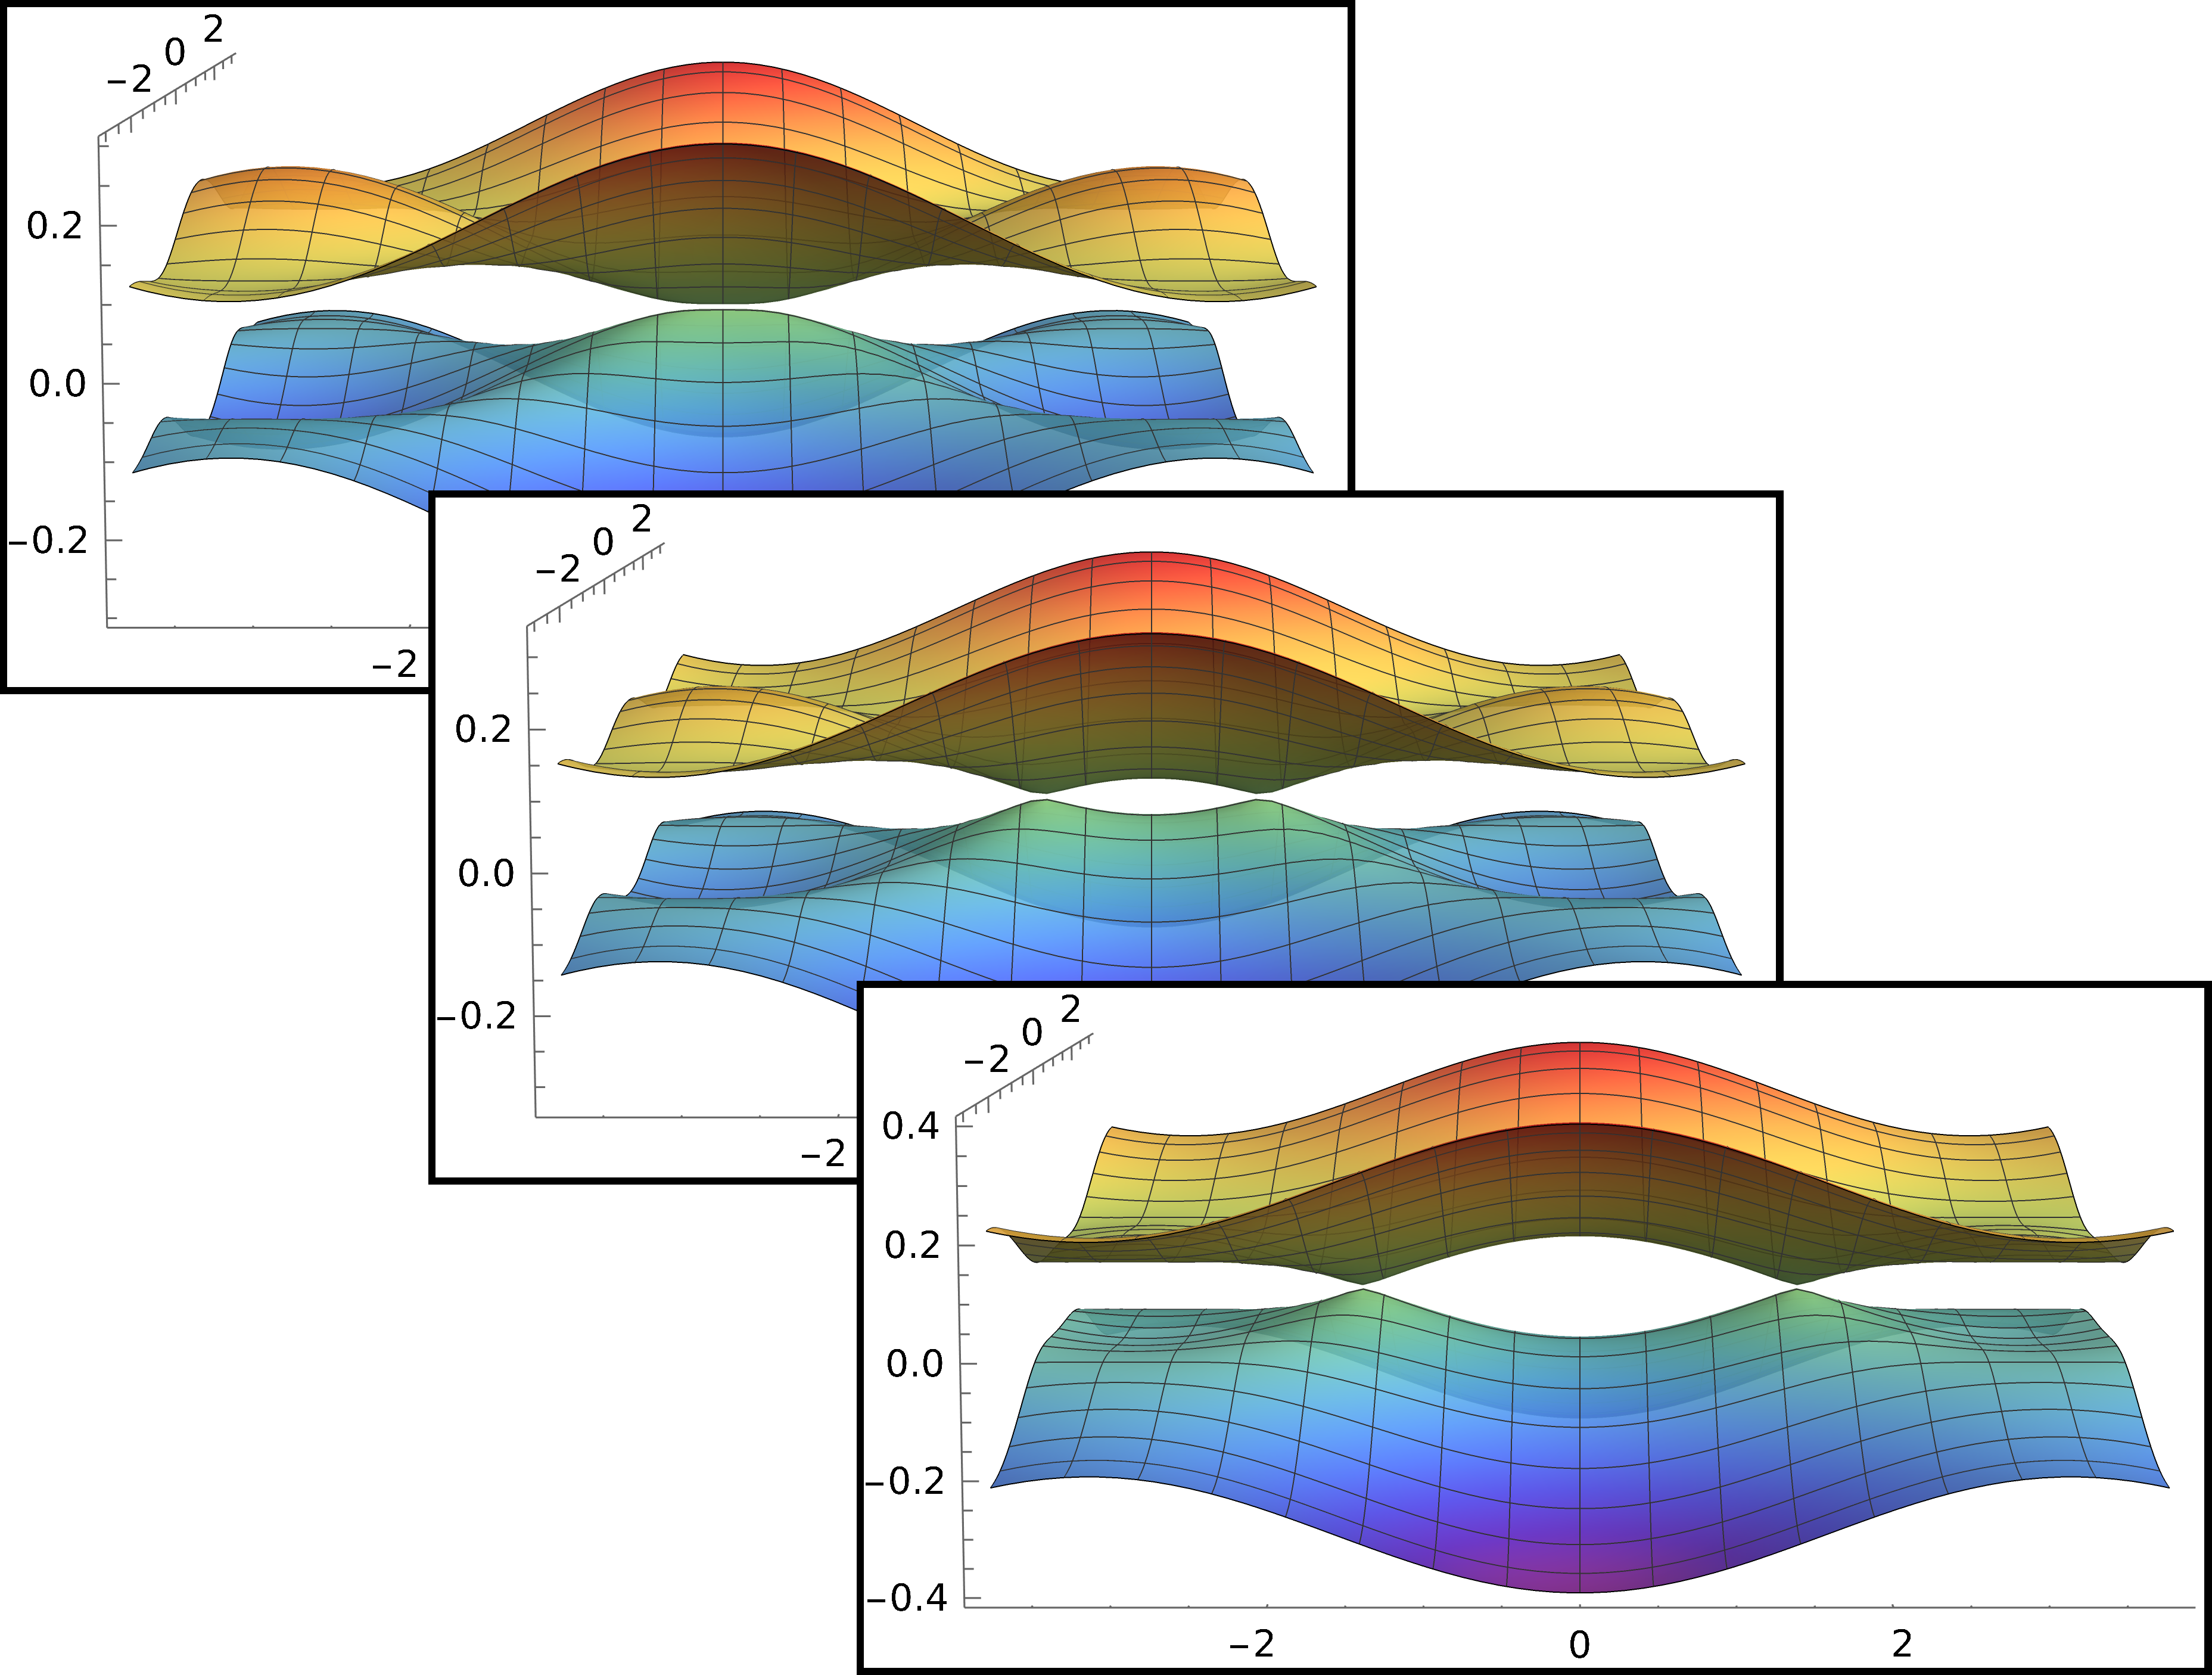
\includegraphics[width=0.7\textwidth]{figures/movetypeiinode}
  \caption{\label{fig:typeii:move-nodes} A Type-II Weyl semimetal with separation between the nodes \(2k_{0} = 0, \pi/2, \pi \).
    See main text for details about the model.}
\end{figure}
